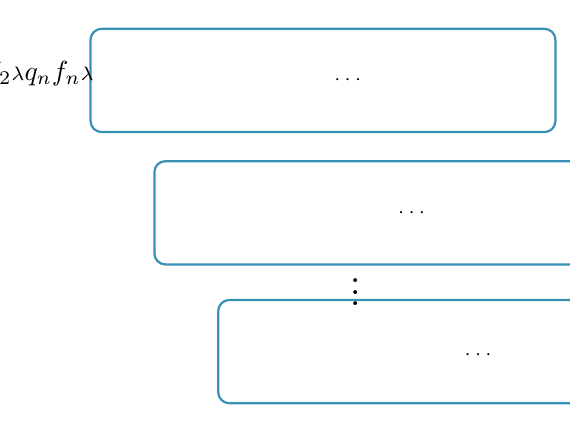
\begin{tikzpicture}[scale=0.82, every node/.style={font=\scriptsize}]

    %-------------------------------------------------
    % společný počáteční stav
    %-------------------------------------------------
    \initialstate<2->{S}{(-1,0)}{$s$}{(-2.0,0.0)}{west}
    \transitionarrow<3->[loop above]{S}{above}{\scriptsize mezera, tab, EOL}{S}

    %-------------------------------------------------
    % větev pro komentář
    %-------------------------------------------------
    % \draw<3->[green!60!black, thick, rounded corners]
    %     (-1.15,-2.55) rectangle (1.20,-1.75);

    \state<3->{C1}{(-1.0,-1.80)}{$c_1$}
    \acceptingstate<3->{C2}{(-1.0,-3.60)}{$c_2$}

    \transitionarrow<3->{S}{left}{\scriptsize zač. komentáře}{C1}
    \transitionarrow<3->[loop right]{C1}{below}{\scriptsize obsah}{C1}
    \transitionarrow<3->{C1}{right}{\scriptsize konec}{C2}
    \transitionarrow<3->[bend left=70]{C2}{left}{\scriptsize přeskočit}{S}

    %-------------------------------------------------
    % T1
    %-------------------------------------------------
    \draw<2->[cyan!70!black, thick, rounded corners]
        (3.00,0.8) rectangle (10.20,-0.80);

    \node<2->[text=cyan!50!black]
        at (10.60,0.0) {$T_1$};

    \state<2->{Q1}{(4.10,0)}{$q_1$}
    \node<2-> (T1dots) at (6.60,0) {\(\cdots\)};
    \acceptingstate<2->{F1}{(9.10,0)}{$f_1$}

    \transitionarrow<2->{S}{above}{\scriptsize \(\lambda\)}{Q1}
    \transitionarrow<2->{Q1}{above}{}{T1dots}
    \transitionarrow<2->{T1dots}{above}{}{F1}

    %-------------------------------------------------
    % T2
    %-------------------------------------------------
    \draw<2->[cyan!70!black, thick, rounded corners]
        (3.00,-1.25) rectangle (10.20,-2.85);

    \node<2->[text=cyan!50!black]
        at (10.60,-2.05) {$T_2$};

    \state<2->{Q2}{(4.10,-2.05)}{$q_2$}
    \node<2-> (T2dots) at (6.60,-2.05) {\(\cdots\)};
    \acceptingstate<2->{F2}{(9.10,-2.05)}{$f_2$}

    \transitionarrow<2->{S}{above}{\scriptsize \(\lambda\)}{Q2}
    \transitionarrow<2->{Q2}{above}{}{T2dots}
    \transitionarrow<2->{T2dots}{above}{}{F2}

    %-------------------------------------------------
    % Tn
    %-------------------------------------------------
    \draw<2->[cyan!70!black, thick, rounded corners]
        (3.00,-3.40) rectangle (10.20,-5.00);

    \node<2->[text=cyan!50!black]
        at (10.60,-4.20) {$T_n$};

    \state<2->{Qn}{(4.10,-4.25)}{$q_n$}
    \node<2-> (Tndots) at (6.60,-4.25) {\(\cdots\)};
    \acceptingstate<2->{Fn}{(9.10,-4.25)}{$f_n$}

    \transitionarrow<2->{S}{above}{\scriptsize \(\lambda\)}{Qn}
    \transitionarrow<2->{Qn}{above}{}{Tndots}
    \transitionarrow<2->{Tndots}{above}{}{Fn}

    %-------------------------------------------------
    % naznačení dalších větví
    %-------------------------------------------------
    \node<2->[font=\Large] at (4.05,-3.15) {\(\vdots\)};

\end{tikzpicture}
